\documentclass[tikz,border=5pt,png]{standalone}
\usepackage{tikz}
\usetikzlibrary{shapes,backgrounds,calc,positioning}
\usepackage[utf8]{inputenc}
\usepackage[T1]{fontenc}
\renewcommand{\familydefault}{\sfdefault}

\begin{document}
	
	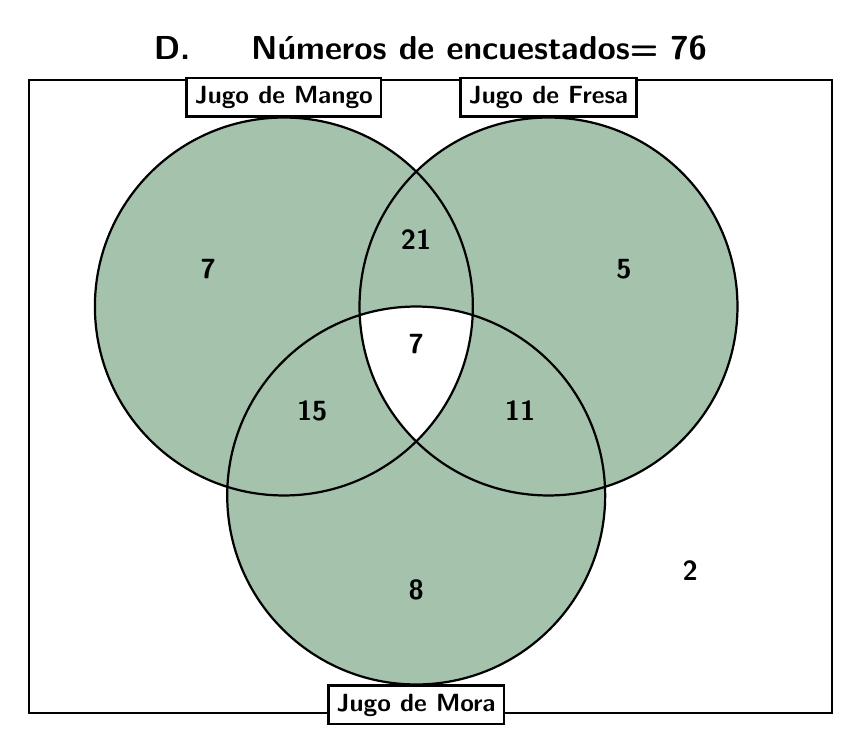
\begin{tikzpicture}[thick, scale=1.2]
		% Definición de colores
		\definecolor{shadedregion}{RGB}{165, 194, 173} % Verde grisáceo de la imagen
		\definecolor{labelbox}{RGB}{255, 255, 255} % Blanco para fondo de etiquetas
		
		% Coordenadas de los centros de los círculos y radio
		\coordinate (M) at (-0.8, 0.8); % Mango (Arriba Izquierda)
		\coordinate (F) at (2.0, 0.8);  % Fresa (Arriba Derecha)
		\coordinate (Mo) at (0.6, -1.2); % Mora (Abajo)
		\def\R{2.0} % Radio de los círculos
		
		% --- Sombreado para la Imagen D ---
		% La región sombreada es la UNIÓN de los tres conjuntos,
		% EXCLUYENDO la intersección común de los tres (el centro).
		
		% 1. Primero, rellenamos la unión de los tres círculos.
		\begin{scope}[on background layer]
			\fill[shadedregion] (M) circle (\R);
			\fill[shadedregion] (F) circle (\R);
			\fill[shadedregion] (Mo) circle (\R);
		\end{scope}
		
		% 2. Luego, rellenamos la intersección central con BLANCO.
		% Usamos 'clip' para aislar la región central.
		\begin{scope}
			% Recortamos al círculo de Mango
			\clip (M) circle (\R);
			% Recortamos al círculo de Fresa (ahora estamos en la intersección M y F)
			\clip (F) circle (\R);
			% Rellenamos la parte del círculo de Mora que está en esa intersección.
			\fill[white] (Mo) circle (\R);
		\end{scope}
		
		% --- Contornos de los Círculos ---
		\draw (M) circle (\R);
		\draw (F) circle (\R);
		\draw (Mo) circle (\R);
		
		% --- Conjunto Universal (Marco) ---
		\draw (-3.5, -3.5) rectangle (5.0, 3.2);
		
		% --- Título ---
		\node[anchor=south, font=\bfseries\large, align=center] at (0.75, 3.3) {D. \hspace{1em} Números de encuestados= 76};
		
		% --- Etiquetas de los Conjuntos ---
		\tikzset{setlabel/.style={draw, fill=labelbox, font=\bfseries\small, inner sep=3pt}}
		\node[setlabel, anchor=south] at ($(M) + (0, \R)$) {Jugo de Mango};
		\node[setlabel, anchor=south] at ($(F) + (0, \R)$) {Jugo de Fresa};
		\node[setlabel, anchor=north] at ($(Mo) - (0, \R)$) {Jugo de Mora};
		
		% --- Números (Datos) ---
		\node[font=\bfseries] at (-1.6, 1.2) {7};  % Solo Mango (Sombreado)
		\node[font=\bfseries] at (2.8, 1.2) {5};   % Solo Fresa (Sombreado)
		\node[font=\bfseries] at (0.6, -2.2) {8};  % Solo Mora (Sombreado)
		\node[font=\bfseries] at (0.6, 1.5) {21};  % Mango y Fresa (Sombreado)
		\node[font=\bfseries] at (-0.5, -0.3) {15}; % Mango y Mora (Sombreado)
		\node[font=\bfseries] at (1.7, -0.3) {11};  % Fresa y Mora (Sombreado)
		\node[font=\bfseries] at (0.6, 0.4) {7};   % Los tres (BLANCO)
		\node[font=\bfseries] at (3.5, -2.0) {2};   % Fuera
		
	\end{tikzpicture}
	
\end{document}